% Options for packages loaded elsewhere
\PassOptionsToPackage{unicode}{hyperref}
\PassOptionsToPackage{hyphens}{url}
\PassOptionsToPackage{dvipsnames,svgnames,x11names}{xcolor}
\documentclass[
  10pt,
  a4paper,
]{article}
\usepackage{xcolor}
\usepackage[margin=0.8in]{geometry}
\usepackage{amsmath,amssymb}
\setcounter{secnumdepth}{-\maxdimen} % remove section numbering
\usepackage{iftex}
\ifPDFTeX
  \usepackage[T1]{fontenc}
  \usepackage[utf8]{inputenc}
  \usepackage{textcomp} % provide euro and other symbols
\else % if luatex or xetex
  \usepackage{unicode-math} % this also loads fontspec
  \defaultfontfeatures{Scale=MatchLowercase}
  \defaultfontfeatures[\rmfamily]{Ligatures=TeX,Scale=1}
\fi
\usepackage[]{newtxtext}
\ifPDFTeX\else
  % xetex/luatex font selection
\fi
% Use upquote if available, for straight quotes in verbatim environments
\IfFileExists{upquote.sty}{\usepackage{upquote}}{}
\IfFileExists{microtype.sty}{% use microtype if available
  \usepackage[]{microtype}
  \UseMicrotypeSet[protrusion]{basicmath} % disable protrusion for tt fonts
}{}
\makeatletter
\@ifundefined{KOMAClassName}{% if non-KOMA class
  \IfFileExists{parskip.sty}{%
    \usepackage{parskip}
  }{% else
    \setlength{\parindent}{0pt}
    \setlength{\parskip}{6pt plus 2pt minus 1pt}}
}{% if KOMA class
  \KOMAoptions{parskip=half}}
\makeatother
\usepackage{longtable,booktabs,array}
\usepackage{caption}
\captionsetup[table]{skip=6pt}
\newcounter{none} % for unnumbered tables
\usepackage{calc} % for calculating minipage widths
% Correct order of tables after \paragraph or \subparagraph
\usepackage{etoolbox}
\makeatletter
\patchcmd\longtable{\par}{\if@noskipsec\mbox{}\fi\par}{}{}
\makeatother
\setlength{\emergencystretch}{3em} % prevent overfull lines
\providecommand{\tightlist}{%
  \setlength{\itemsep}{0pt}\setlength{\parskip}{0pt}}

\usepackage{graphicx}
\usepackage{xurl}
\usepackage{microtype}
\usepackage{fancyhdr}
\usepackage{titlesec}
\usepackage{caption}
\usepackage{fvextra}
\usepackage{placeins}
\usepackage{needspace}
\definecolor{ink}{HTML}{173B50}
\definecolor{linkblue}{HTML}{245C75}
\captionsetup{font=small,labelfont={bf,color=ink},labelsep=period}
\titleformat{\section}{\large\bfseries\color{ink}}{}{0pt}{}
\titleformat{\subsection}{\normalsize\bfseries}{}{0pt}{}
\titlespacing*{\section}{0pt}{14pt}{6pt}
\titlespacing*{\subsection}{0pt}{10pt}{4pt}
\pagestyle{fancy}\fancyhf{}
\fancyhead[L]{\small\sffamily\color{ink}FungalLink v2}
\fancyhead[R]{\small\sffamily Preprint}
\fancyfoot[C]{\small\thepage}
\setlength{\headheight}{14pt}
\renewcommand{\headrulewidth}{0.3pt}
\setlength{\parindent}{0pt}
\setlength{\parskip}{5pt plus 1pt}
\setlength{\emergencystretch}{3em}
\setcounter{topnumber}{2}\setcounter{bottomnumber}{2}
\renewcommand{\topfraction}{0.9}\renewcommand{\textfraction}{0.08}
\renewcommand{\floatpagefraction}{0.75}
\AtBeginEnvironment{longtable}{\small}
\RecustomVerbatimEnvironment{verbatim}{Verbatim}{breaklines=true,fontsize=\footnotesize}
\AtBeginDocument{\hypersetup{colorlinks=true,linkcolor=linkblue,urlcolor=linkblue,citecolor=linkblue,breaklinks=true}}
\usepackage{bookmark}
\IfFileExists{xurl.sty}{\usepackage{xurl}}{} % add URL line breaks if available
\urlstyle{same}
% fallback for those not using the hyperref driver hyperxmp:
\makeatletter
\@ifundefined{xmpquote}{\newcommand{\xmpquote}[1]{#1}}{}
\makeatother
\hypersetup{
  colorlinks=true,
  linkcolor={Maroon},
  filecolor={Maroon},
  citecolor={Blue},
  urlcolor={linkblue},
  pdfcreator={LaTeX via pandoc}}

\author{}
\date{}

\begin{document}

\begin{center}{\LARGE\bfseries\color{ink}Comparative results\par}\vspace{6pt}
{\large FungalLink v2}\\[4pt]
Vin Vomero\\[4pt]
11 October 2026\end{center}
\vspace{8pt}
\renewcommand{\thefigure}{S\arabic{figure}}

Companion to the FungalLink v2 Data Descriptor. Tables 1--3 retain their exact values and analysis identities. The six-product experiment, nine-target amendment, family-view extensions, partial diagnostics and assembly-matched comparison are separate analyses. References {[}1--16{]} refer to the main article.

\subsection{Initial six-product analysis}\label{initial-six-product-analysis}

The following results describe only the frozen experiment preceding the seven additional admissions on 7 October 2026. All four deterministic workflows returned complete rankings for its five queries on every roster, yielding 72 runs. Conditional and end-to-end estimates were therefore identical. Table 1 and Figure S1 report initial six-target results; the full \href{https://github.com/vinvomero/fungallink-benchmark/blob/main/manuscript/initial-comparison-results-2026-10-07.tsv}{results table} retains roster, query and evidence-stratum detail.

Table 1. Primary retrieval estimates. MRR is mean expected reciprocal rank. Random values are exact expectations. Fractional hit estimates reflect score ties and are not counts of successful queries.

{\def\LTcaptype{none} % do not increment counter
\begin{longtable}[]{@{}
  >{\raggedright\arraybackslash}p{(\linewidth - 12\tabcolsep) * \real{0.1111}}
  >{\raggedleft\arraybackslash}p{(\linewidth - 12\tabcolsep) * \real{0.1481}}
  >{\raggedleft\arraybackslash}p{(\linewidth - 12\tabcolsep) * \real{0.1481}}
  >{\raggedleft\arraybackslash}p{(\linewidth - 12\tabcolsep) * \real{0.1481}}
  >{\raggedleft\arraybackslash}p{(\linewidth - 12\tabcolsep) * \real{0.1481}}
  >{\raggedleft\arraybackslash}p{(\linewidth - 12\tabcolsep) * \real{0.1481}}
  >{\raggedleft\arraybackslash}p{(\linewidth - 12\tabcolsep) * \real{0.1481}}@{}}
\toprule\noalign{}
\begin{minipage}[b]{\linewidth}\raggedright
Workflow
\end{minipage} & \begin{minipage}[b]{\linewidth}\raggedleft
\href{mailto:Hit@1}{\nolinkurl{Hit@1}}
\end{minipage} & \begin{minipage}[b]{\linewidth}\raggedleft
\href{mailto:Hit@10}{\nolinkurl{Hit@10}}
\end{minipage} & \begin{minipage}[b]{\linewidth}\raggedleft
\href{mailto:Hit@100}{\nolinkurl{Hit@100}}
\end{minipage} & \begin{minipage}[b]{\linewidth}\raggedleft
MRR
\end{minipage} & \begin{minipage}[b]{\linewidth}\raggedleft
Product \href{mailto:recovery@10}{\nolinkurl{recovery@10}}
\end{minipage} & \begin{minipage}[b]{\linewidth}\raggedleft
All \href{mailto:products@10}{\nolinkurl{products@10}}
\end{minipage} \\
\midrule\noalign{}
\endhead
\bottomrule\noalign{}
\endlastfoot
Global prevalence & 0 & 0 & 0 & 0.001095 & 0 & 0 \\
Uniform random & 0.000128 & 0.001285 & 0.012827 & 0.001206 & 0.001071 & 0.000857 \\
Prevalence difference & 0 & 0.487302 & 1 & 0.132674 & 0.465079 & 0.442857 \\
Raw Metcalf & 0.050397 & 0.853968 & 1 & 0.252240 & 0.753968 & 0.653968 \\
Standardized Metcalf & 0.014286 & 0.615079 & 1 & 0.192873 & 0.590079 & 0.565079 \\
\end{longtable}
}

For pestalamides, raw Metcalf placed feature 810 within ranks 1--8 and feature 725 within ranks 41--49. \href{mailto:Hit@10}{\nolinkurl{Hit@10}} was consequently 1, but product \href{mailto:recovery@10}{\nolinkurl{recovery@10}} was 0.5 and all-products \href{mailto:recovery@10}{\nolinkurl{recovery@10}} was 0. Standardization placed these features within ranks 9--16 and 17--25, giving expected \href{mailto:hit@10}{\nolinkurl{hit@10}} of 0.25 and product \href{mailto:recovery@10}{\nolinkurl{recovery@10}} of 0.125. Both products were recovered by rank 100 under each query-dependent workflow. The rank ranges describe ties, not sampling uncertainty.

The directly supported stratum consists of that single two-product query. Across the four reference-supported queries, \href{mailto:hit@10}{\nolinkurl{hit@10}} was 0.817460 for raw Metcalf, 0.706349 for standardized Metcalf and 0.553571 for prevalence difference. These strata remain subsets of the same analysis group.

Across all rosters, raw-Metcalf \href{mailto:hit@10}{\nolinkurl{hit@10}} ranged from 0.767857 to 0.853968, standardized Metcalf from 0.577579 to 0.697243, and prevalence difference from 0.465079 to 0.590476. Raw Metcalf had the largest \href{mailto:hit@10}{\nolinkurl{hit@10}} on every roster, but standardized Metcalf had larger MRR on the three-media restrictions of assembly choices 01 and 02: 0.218561 versus 0.212852. All query-dependent workflows recovered every supported product by rank 100 on every roster. These overlapping roster comparisons measure sensitivity to composition, without isolating causal effects of medium or dependence.

The shared random simulation achieved its precision criterion after 4,000 repetitions, with maximum MCSE 0.0008148165. Simulated \href{mailto:hit@10}{\nolinkurl{hit@10}} was 0.001200 and MRR 0.001266. Scoring and evaluation of the deterministic runs took 55.60 seconds in total, excluding setup and serialization; the random run took 358.55 seconds elapsed. These are recorded execution costs, not isolated method benchmarks.

A separate numerical audit checked all 186,780 primary candidate scores and 80 primary any-hit/reciprocal-rank metrics without baseline or evaluator helpers. A clean-directory same-host rerun under Python 3.13.5 with site packages disabled (\texttt{python\ -S}) reproduced all 72 deterministic runs exactly as parsed JSON, including scores, audits, statuses and evaluator fields. The automated reproducer was not an independent researcher, and the 4,000-repeat Monte Carlo simulation was not rerun.

A subsequent private source rebuild used a new local Git snapshot and clean clone, cached publisher-workbook bytes and hash-pinned curation inputs. In 121.8 seconds, all 20 output files from four source stages matched exactly, the complete released input file was byte-identical, and expanded nine-target gold matched as parsed JSON. All four primary deterministic workflows reproduced their complete rankings and expanded evaluations exactly. This run used the same host and agent with isolated Python imports and pinned existing dependency files. It did not rerun the other 17 rosters or Monte Carlo control, reproduce biological adjudication, or derive the historical sample and family mappings entirely from public evidence. The \href{https://github.com/vinvomero/fungallink-benchmark/blob/main/docs/release/clean-source-reproduction-2026-10-07.md}{source-rebuild report} and \href{https://github.com/vinvomero/fungallink-benchmark/blob/main/data/processed/clean-source-reproduction-2026-10-07/host-verification.json}{host verification} define the checked stages and input boundary.

\subsection{Nine-target retrospective amendment}\label{nine-target-retrospective-amendment}

After the initial analysis, the evidence-based admissions supported a separately versioned nine-target evaluation, \nolinkurl{source-selected-gcf-expanded-labels-v2}. It added notoamide E (feature 4182) and the structure-putative pestalamide E/F-associated features (1950 and 895). The notoamide query now contains two targets and the pestalamide query four; three other queries each retain one. These are nine supported product or measured-feature targets at their declared chemical resolution, not nine fully elucidated structures or independent pathways.

The attributed amendment was recorded before inspecting the added targets' ranks, but the original six-product results were already known. All 72 ranking files were reused byte-for-byte, with unchanged inputs, scores, method version 0.1.0, evaluator and 18 rosters. Only the positive sets and their evaluations changed. Every query retained complete coverage. This is a retrospective evidence-based extension, not a blind prospective test; ilicicolin H and the FAC cases were not scored in that comparison.

Table 2. Primary nine-target amendment. Metrics are query-averaged expectations under score ties. Random values are exact expectations; no new Monte Carlo run was performed.

{\def\LTcaptype{none} % do not increment counter
\begin{longtable}[]{@{}
  >{\raggedright\arraybackslash}p{(\linewidth - 12\tabcolsep) * \real{0.1111}}
  >{\raggedleft\arraybackslash}p{(\linewidth - 12\tabcolsep) * \real{0.1481}}
  >{\raggedleft\arraybackslash}p{(\linewidth - 12\tabcolsep) * \real{0.1481}}
  >{\raggedleft\arraybackslash}p{(\linewidth - 12\tabcolsep) * \real{0.1481}}
  >{\raggedleft\arraybackslash}p{(\linewidth - 12\tabcolsep) * \real{0.1481}}
  >{\raggedleft\arraybackslash}p{(\linewidth - 12\tabcolsep) * \real{0.1481}}
  >{\raggedleft\arraybackslash}p{(\linewidth - 12\tabcolsep) * \real{0.1481}}@{}}
\toprule\noalign{}
\begin{minipage}[b]{\linewidth}\raggedright
Workflow
\end{minipage} & \begin{minipage}[b]{\linewidth}\raggedleft
\href{mailto:Hit@10}{\nolinkurl{Hit@10}}
\end{minipage} & \begin{minipage}[b]{\linewidth}\raggedleft
Product \href{mailto:recovery@10}{\nolinkurl{recovery@10}}
\end{minipage} & \begin{minipage}[b]{\linewidth}\raggedleft
All \href{mailto:products@10}{\nolinkurl{products@10}}
\end{minipage} & \begin{minipage}[b]{\linewidth}\raggedleft
Product \href{mailto:recovery@100}{\nolinkurl{recovery@100}}
\end{minipage} & \begin{minipage}[b]{\linewidth}\raggedleft
All \href{mailto:products@100}{\nolinkurl{products@100}}
\end{minipage} & \begin{minipage}[b]{\linewidth}\raggedleft
MRR
\end{minipage} \\
\midrule\noalign{}
\endhead
\bottomrule\noalign{}
\endlastfoot
Global prevalence & 0.000000 & 0.000000 & 0.000000 & 0.000000 & 0.000000 & 0.001107 \\
Uniform random (exact) & 0.001926 & 0.001071 & 0.000643 & 0.010708 & 0.006447 & 0.001674 \\
Prevalence difference & 0.487302 & 0.353968 & 0.242857 & 0.900000 & 0.800000 & 0.132674 \\
Raw Metcalf & 0.853968 & 0.603968 & 0.453968 & 0.966667 & 0.933333 & 0.252240 \\
Standardized Metcalf & 0.615079 & 0.477579 & 0.365079 & 0.915000 & 0.803846 & 0.192873 \\
\end{longtable}
}

For the three query-dependent workflows, primary any-hit retrieval and MRR were unchanged, while recovery of all supported targets declined. At rank 100, mean all-products recovery was 0.933333 for raw Metcalf, 0.803846 for standardized Metcalf and 0.800000 for prevalence difference, compared with 1 for each in the six-product analysis. At rank 10, raw Metcalf retained any-hit retrieval of 0.853968 while its mean product recovery fell from 0.753968 to 0.603968 and all-products recovery from 0.653968 to 0.453968. Thus an unchanged early hit can conceal missed products of the same query.

Figure S2 shows sensitivity to the observation roster. Figure S3 traces each target through its exact rank interval, including the three added labels. Across the 18 overlapping rosters, all-products \href{mailto:recovery@100}{\nolinkurl{recovery@100}} ranged from 0.753471 to 0.933333 for raw Metcalf, 0.800000 to 1.000000 for standardized Metcalf, and 0.800000 to 0.807973 for prevalence difference. The directly supported stratum remains one query, now with four targets; the reference-supported stratum remains four queries, now with five. All remain in the same conservative analysis group. The \href{https://github.com/vinvomero/fungallink-benchmark/blob/main/manuscript/expanded-label-results-2026-10-07.tsv}{720-row amendment results} retain every query, roster and evidence stratum. Validation checked 18 input projections, 72 successful evaluations and preservation of all 285 original analysis artifacts, without recomputing scores. A separate same-host numerical check recomputed all 3,600 deterministic per-query metric cells from the cached rankings using independent combinatorial code; every cell passed. This automated check does not constitute independent researcher validation.

\subsection{Separate emericellamide family-view extension}\label{separate-emericellamide-family-view-extension}

A further retrospective extension, \nolinkurl{emericellamide-gcf-extension-v1}, evaluated the already-admitted emericellamide A relationship through the fixed source HRPKS\_71 family. The accepted historical locus is a member of that family, but the family representation is broader than the BGC and does not imply production by every member. This declared BGC-to-GCF transformation adds evaluated coverage for one existing relationship, not another biological admission. This extension provides complete evaluation for one additional relationship through a sixth query view. The original five-query positive sets and comparisons remain unchanged.

The extension was frozen before computing its scores, with the earlier five-query results already known. It used the same 9,339 candidates, 18 observation rosters and four deterministic workflows, version 0.1.0. On the primary 105-observation roster, 19 observations are documentary family members and 86 are roster nonmembers. Feature 8468 is the singleton target. Neither roster nonmembership nor the tested family view establishes genomic absence or exclusive biosynthesis.

All 72 runs returned complete rankings. On the primary roster, emericellamide's exact tie-rank intervals were 414--485 for global prevalence, 13--15 for prevalence difference, 27--29 for raw Metcalf and 15--17 for standardized Metcalf. No workflow recovered it within the top ten. The three query-dependent workflows recovered it within the top 100 on every roster; global prevalence did not. Expected reciprocal ranks on the primary roster were 0.002229, 0.071673, 0.035745 and 0.062663, respectively, compared with the exact random expectation of 0.001041.

A separate arithmetic check reconstructed 672,408 scores and 720 metric cells from the frozen inputs and cached outputs. All matched within 1e-12. This same-host numerical verification does not validate the biological assignment independently. The \href{https://github.com/vinvomero/fungallink-benchmark/blob/main/manuscript/emericellamide-extension-results-2026-10-08.md}{extension results and reproduction record} retain the complete roster results. Supporting figures describe the original five-query analyses; this extension is reported separately. Overlapping rosters, source-selected families and one conservative group preclude independent-replicate or significant-winner claims.

\subsection{Separate acetylaszonalenin family-view extension}\label{separate-acetylaszonalenin-family-view-extension}

The separately frozen \nolinkurl{acetylaszonalenin-gcf-extension-v1} evaluates the already-admitted corrected acetylaszonalenin relationship through source family DMAT\_34. A dated evidence correction resolved the earlier exclusion: the sampled historical source display contains all three accepted-core proteins, whereas the contrary coordinates belonged to successor annotation numbering. This correspondence supports the declared family view; full historical-region nucleotide boundaries remain unverified. The assembly contamination flag and unknown locus-specific contamination status remain recorded.

The primary roster contains three documentary family members and 102 nonmembers. The extension uses the same 9,339 candidates, 18 observation rosters and four version-0.1.0 deterministic workflows. The singleton target is feature 2127. DMAT\_34 was selected from the original source association and frozen before this extension's scores were computed; earlier five-query and emericellamide results were already known. Family nonmembership is not verified genomic absence, and membership does not establish production by every member.

All 72 runs returned complete rankings. On the primary roster, prevalence difference and standardized Metcalf ranked the target second, raw Metcalf ranked it 92nd, and global prevalence tied it across ranks 1,389--2,431. Expected reciprocal ranks were 0.500000, 0.500000, 0.010870 and 0.000537, respectively. Across all 18 rosters, prevalence difference and standardized Metcalf recovered the target within ten candidates; raw Metcalf recovered it within 100 but not ten, and global prevalence did not recover it within 100. Exact random expectations remain those of a singleton target among 9,339 candidates.

Separate arithmetic checked 672,408 scores and 720 metric cells against frozen inputs and cached outputs; all matched within 1e-12. This is numerical verification on the same host, not independent biological validation. The \href{https://github.com/vinvomero/fungallink-benchmark/blob/main/manuscript/acetylaszonalenin-extension-results-2026-10-08.md}{extension results and reproduction record} preserve the complete results. Across the original expanded comparison and both separate extensions, 11 of 30 admitted relationships have evaluated coverage through seven query views. Nineteen admitted relationships lack complete evaluated coverage: ilicicolin H, two HEx relationships, one black-yeast-study expression relationship and fifteen FAC-MS relationships, including the seven later valactamide measured-target admissions. Alternative family views do not add biological admissions or independent groups, and the supporting figures retain the original five-query analysis scope.

\subsection{Spectral coverage in two expression experiments}\label{spectral-coverage-in-two-expression-experiments}

Input recovery extended beyond the 11 relationships with complete evaluated coverage. A single black-yeast 6-MSA expression acquisition yielded 1,249 candidate features, of which 291 had selected MS/MS spectra. The separately retained Trichoderma ilicicolin H pool contained 98 candidates and 91 spectra. Neither pool supplied independent-genome variation for the correlation workflows used above. Experimental conditions were not treated as independent genomes.

We generated chemical-superclass inputs using the positive and negative models from the formally versioned Spec2Class software {[}16{]}, available in the \href{https://github.com/VickiPol/Spec2Class/tree/21c6f9433227c689d00549eae25e1fa2d4238fc3}{author repository}. Model files, source revisions, preprocessing and numerical environments were recorded. The positive pipeline reproduced all 100 published example final labels after recovery of a complete author fixture; the CSV version had truncated one peak array. This reproduction checks implementation compatibility, not predictive accuracy on fungal metabolites. Negative predictions covered all 291 supplied spectra. Positive predictions covered 90 of 91 supplied spectra; one had no fragments after the fixed preprocessing rules. The seven Trichoderma candidates without spectra and the empty-spectrum candidate remained uncovered. Unusual or unresolved charge annotations were retained.

A separately declared, reference-aware diagnostic combined the 6-MSA query's transferred T1PKS class with predicted superclasses using the pinned NPLinker class-association table. This broad genomic-class transfer used the known reference and was not a new antiSMASH run or an unseen-pathway evaluation. Scores were available for 291 of 1,249 candidates (23.30\%). The supported target received a score of zero: Spec2Class predicted Triterpenoids, for which the reference table contained no T1PKS association. Ninety-four candidates scored higher, and 197 candidates, including the target, shared its score. The target's rank interval was therefore 95--291 among scored candidates. Allowing the 958 unscored candidates to occupy any positions widened the full-pool interval to 95--1,249. Missing scores were not imputed, and the target result was retained without changing classes or thresholds.

A second predeclared diagnostic used the published PKS-NRPS annotation of TriliA and the retained QM6a reference correspondence for the ilicicolin H query. This literature-derived input was reference-informed, not a blind sequence prediction. The same pinned class-association kernel scored 89 of 98 candidates (90.82\%). One predicted superclass, Isoflavonoids, was absent from the reference table; together with seven missing spectra and one spectrum empty after preprocessing, this left nine candidates unscored. The supported target scored 0.00660066. Fifteen candidates scored higher and six, including the target, tied, giving a scored-only rank interval of 16--21 and conservative full-pool bounds of 16--30. These bounds describe ties and missing outputs, not statistical confidence. No unavailable score was imputed and no vocabulary remapping was used to improve the target rank.

These findings show the limits of the recovered inputs and this class-based workflow. They do not add a complete-output relationship to the evaluated count. The 6-MSA target retains its putative chemical resolution and an unresolved source-intensity discrepancy. The Trichoderma result retains reference exposure and single-background limitations. Both diagnostics remain outside the count of 11 completely evaluated relationships. The \href{https://github.com/vinvomero/fungallink-benchmark/blob/main/manuscript/tables/sixmsa-class-diagnostic-2026-10-09.tsv}{6-MSA results}, \href{https://github.com/vinvomero/fungallink-benchmark/blob/main/manuscript/tables/trichoderma-class-diagnostic-2026-10-11.tsv}{ilicicolin H results}, input protocols and run records preserve the candidate universes, exposure, missing inputs and failed attempts.

\subsection{Comparison on the assembly-matched population}\label{comparison-on-the-assembly-matched-population}

A separately frozen comparison projected the same five source-selected GCF queries, nine supported targets and 9,339 measured candidates onto 66 observations with distinct versioned assemblies. Four deterministic workflows, a BayesTraits dependent-versus-independent binary-character score and exact uniform expectations were evaluated on this identical population. This is a matched method comparison within the existing cohort; it adds no biological relationship or independent analysis group. The earlier 105-observation results are a different population and are not used to attribute changes to phylogeny alone.

The tree used 1,078 protein markers and 551,870 aligned sites. BayesTraits rankings use the declared likelihood-ratio and rate-quotient rule. An initial optimizer failure led to a retrospective, versioned conditional recovery policy: 24 of 7,290 distinct nonconstant query-feature pattern pairs required the alternative-optimizer route. All final pairs passed the unchanged numerical checks. Native fits, selected likelihoods, complete rankings and evaluation arithmetic were reconstructed from retained logs without refitting. This verification establishes numerical consistency, not global optimizer convergence.

Table 3. Assembly-matched comparison on 66 observations. Values are query-averaged expectations under exact score ties; all methods cover all five queries. Products, query identities and observations are distinct counting units. Full-precision per-query and per-product results accompany the table.

{\def\LTcaptype{none} % do not increment counter
\begin{longtable}[]{@{}
  >{\raggedright\arraybackslash}p{(\linewidth - 12\tabcolsep) * \real{0.1111}}
  >{\raggedleft\arraybackslash}p{(\linewidth - 12\tabcolsep) * \real{0.1481}}
  >{\raggedleft\arraybackslash}p{(\linewidth - 12\tabcolsep) * \real{0.1481}}
  >{\raggedleft\arraybackslash}p{(\linewidth - 12\tabcolsep) * \real{0.1481}}
  >{\raggedleft\arraybackslash}p{(\linewidth - 12\tabcolsep) * \real{0.1481}}
  >{\raggedleft\arraybackslash}p{(\linewidth - 12\tabcolsep) * \real{0.1481}}
  >{\raggedleft\arraybackslash}p{(\linewidth - 12\tabcolsep) * \real{0.1481}}@{}}
\toprule\noalign{}
\begin{minipage}[b]{\linewidth}\raggedright
Workflow
\end{minipage} & \begin{minipage}[b]{\linewidth}\raggedleft
\href{mailto:Hit@10}{\nolinkurl{Hit@10}}
\end{minipage} & \begin{minipage}[b]{\linewidth}\raggedleft
Product \href{mailto:recovery@10}{\nolinkurl{recovery@10}}
\end{minipage} & \begin{minipage}[b]{\linewidth}\raggedleft
All \href{mailto:products@10}{\nolinkurl{products@10}}
\end{minipage} & \begin{minipage}[b]{\linewidth}\raggedleft
Product \href{mailto:recovery@100}{\nolinkurl{recovery@100}}
\end{minipage} & \begin{minipage}[b]{\linewidth}\raggedleft
All \href{mailto:products@100}{\nolinkurl{products@100}}
\end{minipage} & \begin{minipage}[b]{\linewidth}\raggedleft
MRR
\end{minipage} \\
\midrule\noalign{}
\endhead
\bottomrule\noalign{}
\endlastfoot
Global prevalence & 0.000000 & 0.000000 & 0.000000 & 0.000000 & 0.000000 & 0.000985 \\
Prevalence difference & 0.311111 & 0.227778 & 0.200000 & 0.550000 & 0.412319 & 0.199501 \\
Raw Metcalf & 0.494222 & 0.428054 & 0.400348 & 0.657274 & 0.518852 & 0.255842 \\
Standardized Metcalf & 0.528410 & 0.436601 & 0.400348 & 0.620715 & 0.457655 & 0.264953 \\
BayesTraits directed LRT & 0.255556 & 0.213889 & 0.200000 & 0.782353 & 0.729412 & 0.075740 \\
Uniform random (exact) & 0.001926 & 0.001071 & 0.000643 & 0.010708 & 0.006447 & 0.001674 \\
\end{longtable}
}

BayesTraits had lower early retrieval than raw or standardized Metcalf: \href{mailto:Hit@10}{\nolinkurl{Hit@10}} was 0.255556 versus 0.494222 and 0.528410, and MRR was 0.075740 versus 0.255842 and 0.264953. At rank 100, BayesTraits had higher mean product recovery (0.782353 versus 0.657274 and 0.620715) and all-products recovery (0.729412 versus 0.518852 and 0.457655). Conditional on the fixed tree and model, the method therefore changed the balance between early retrieval and broader product recovery on this population; it did not improve every metric. Its first-positive rank bounds were 5--6 for NRPSLIKE\_59, 6--23 for NRPSPKS\_85, 15--76 for NRPS\_66 and 11--14 for TERPENE\_40. The NRPKS\_18 target remained in a broad tie spanning ranks 776--9,339.

These descriptive results come from five selected queries in one conservative analysis group. The unpartitioned fixed-model tree, midpoint rooting, absence of branch-support resampling and composition-test failures in 65 of 66 sequences limit phylogenetic interpretation. Documentary family nonmembership is not experimentally verified genomic absence. The optimizer amendment was retrospective. Neither this comparison nor the numerical audit establishes statistical superiority, independent biological validation or unseen-pathway performance. The \href{https://github.com/vinvomero/fungallink-benchmark/blob/main/manuscript/tables/phylogeny-comparison-v2/README.md}{verified tables}, their \href{https://github.com/vinvomero/fungallink-benchmark/blob/main/manuscript/tables/phylogeny-comparison-v2/receipt.json}{export receipt} and Supplementary Methods preserve the full scope.

\section{Supporting performance figures}\label{supporting-performance-figures}

\begin{figure}[!htbp]
\centering
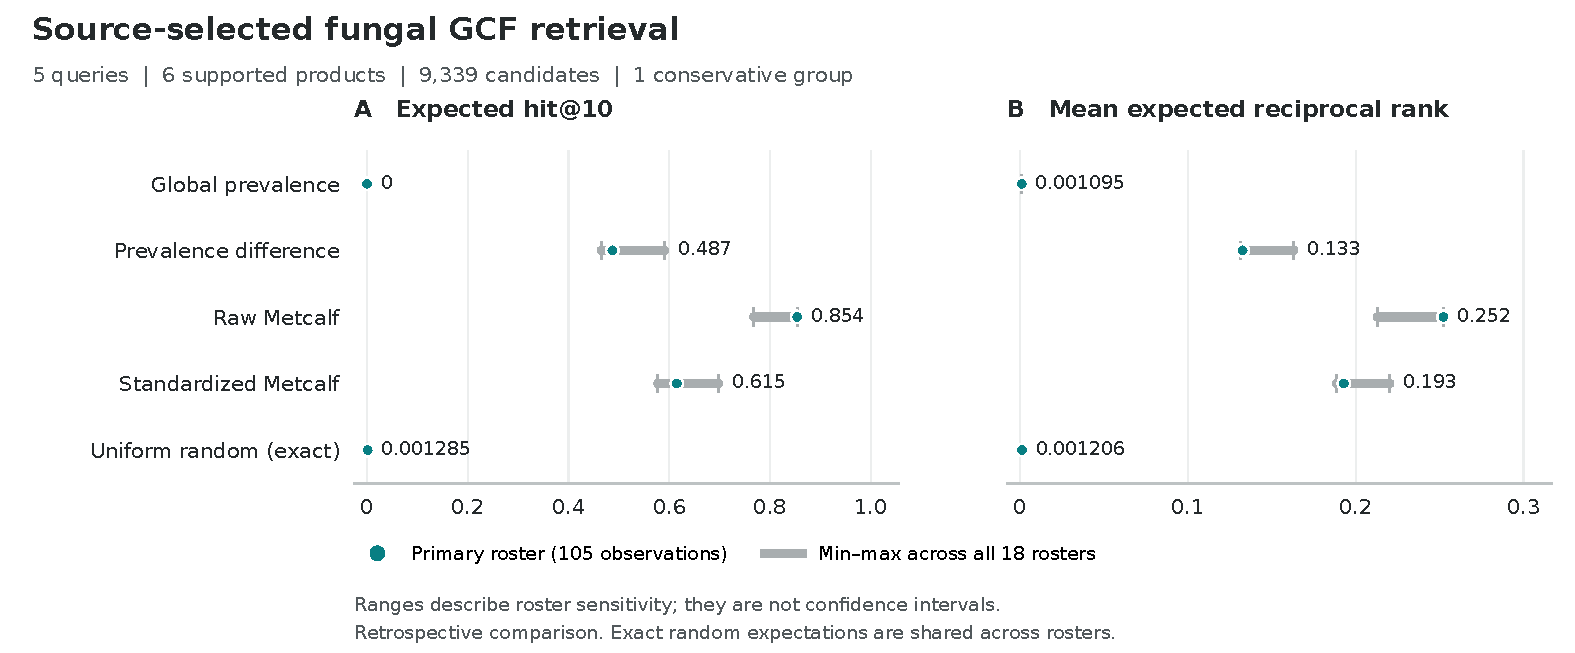
\includegraphics[width=\linewidth,height=0.62\textheight,keepaspectratio]{figures/Figure-S1.pdf}
\caption{Expected hit@10 and MRR for five GCF queries, six products and 9,339 candidates. Teal points mark the primary 105-observation roster; gray segments span all 18 overlapping rosters. Ranges are sensitivity summaries, not confidence intervals. Random points show exact expectations. Ties receive expected credit, and all deterministic workflows covered every query. Source selection and one conservative analysis group preclude a significance or winner claim.}
\label{fig:S1}
\end{figure}

\FloatBarrier

\clearpage

\begin{figure}[!htbp]
\centering
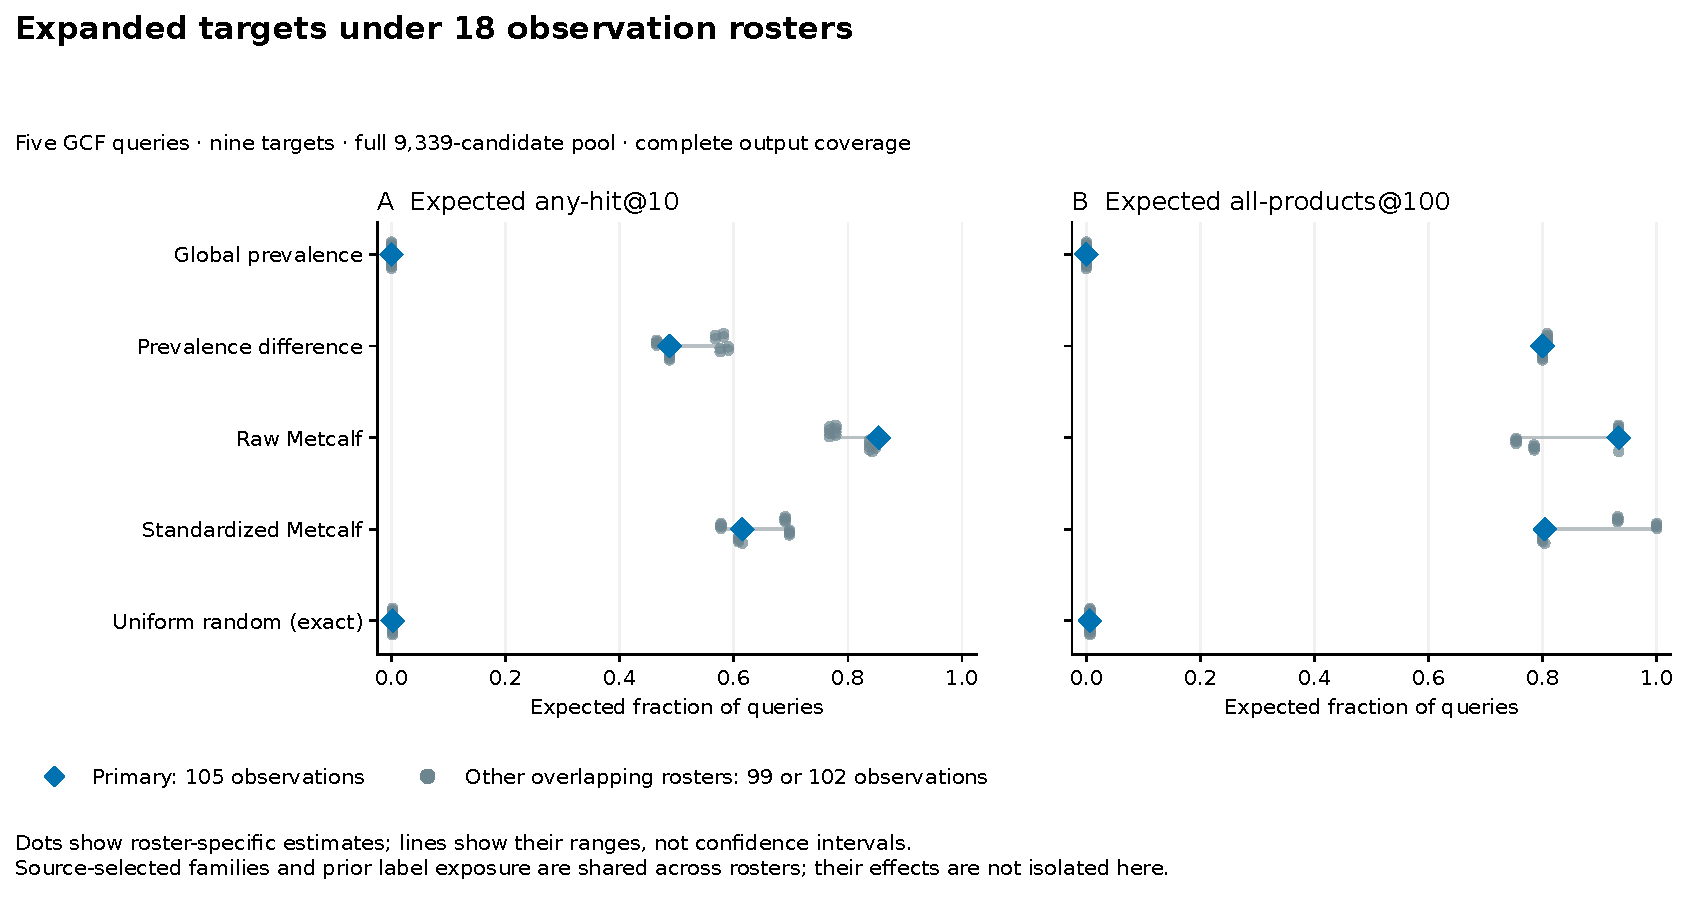
\includegraphics[width=\linewidth,height=0.62\textheight,keepaspectratio]{figures/Figure-S2.pdf}
\caption{Expanded-target sensitivity to the observation roster. Expected any-hit retrieval at rank 10 (A) and joint recovery of all supported targets at rank 100 (B) are shown for the nine-target, five-query amendment. Diamonds mark the primary 105-observation roster. Circles show the other 17 overlapping rosters: the 102-observation three-media restriction, eight 102-observation assembly-representative choices, and their eight 99-observation three-media restrictions. Vertical offsets separate overlapping symbols and carry no numerical meaning. Horizontal lines span the observed roster-specific estimates; they are not biological confidence intervals. Exact score ties receive uniform-order expectation, and the random control is analytic. All queries have complete candidate output coverage. The 9,339-candidate universe, expanded gold, source-selected family definitions and permitted feature-only inputs are fixed across rosters. The plot measures roster sensitivity; it does not estimate the effects of source selection, candidate filtering, prior exposure or adding spectral inputs. Historical label exposure and the source-selected retrospective design limit interpretation across every roster. No comparison of independent biological replicates, significance test or method-superiority claim is implied.}
\label{fig:S2}
\end{figure}

\FloatBarrier

\clearpage

\begin{figure}[!htbp]
\centering
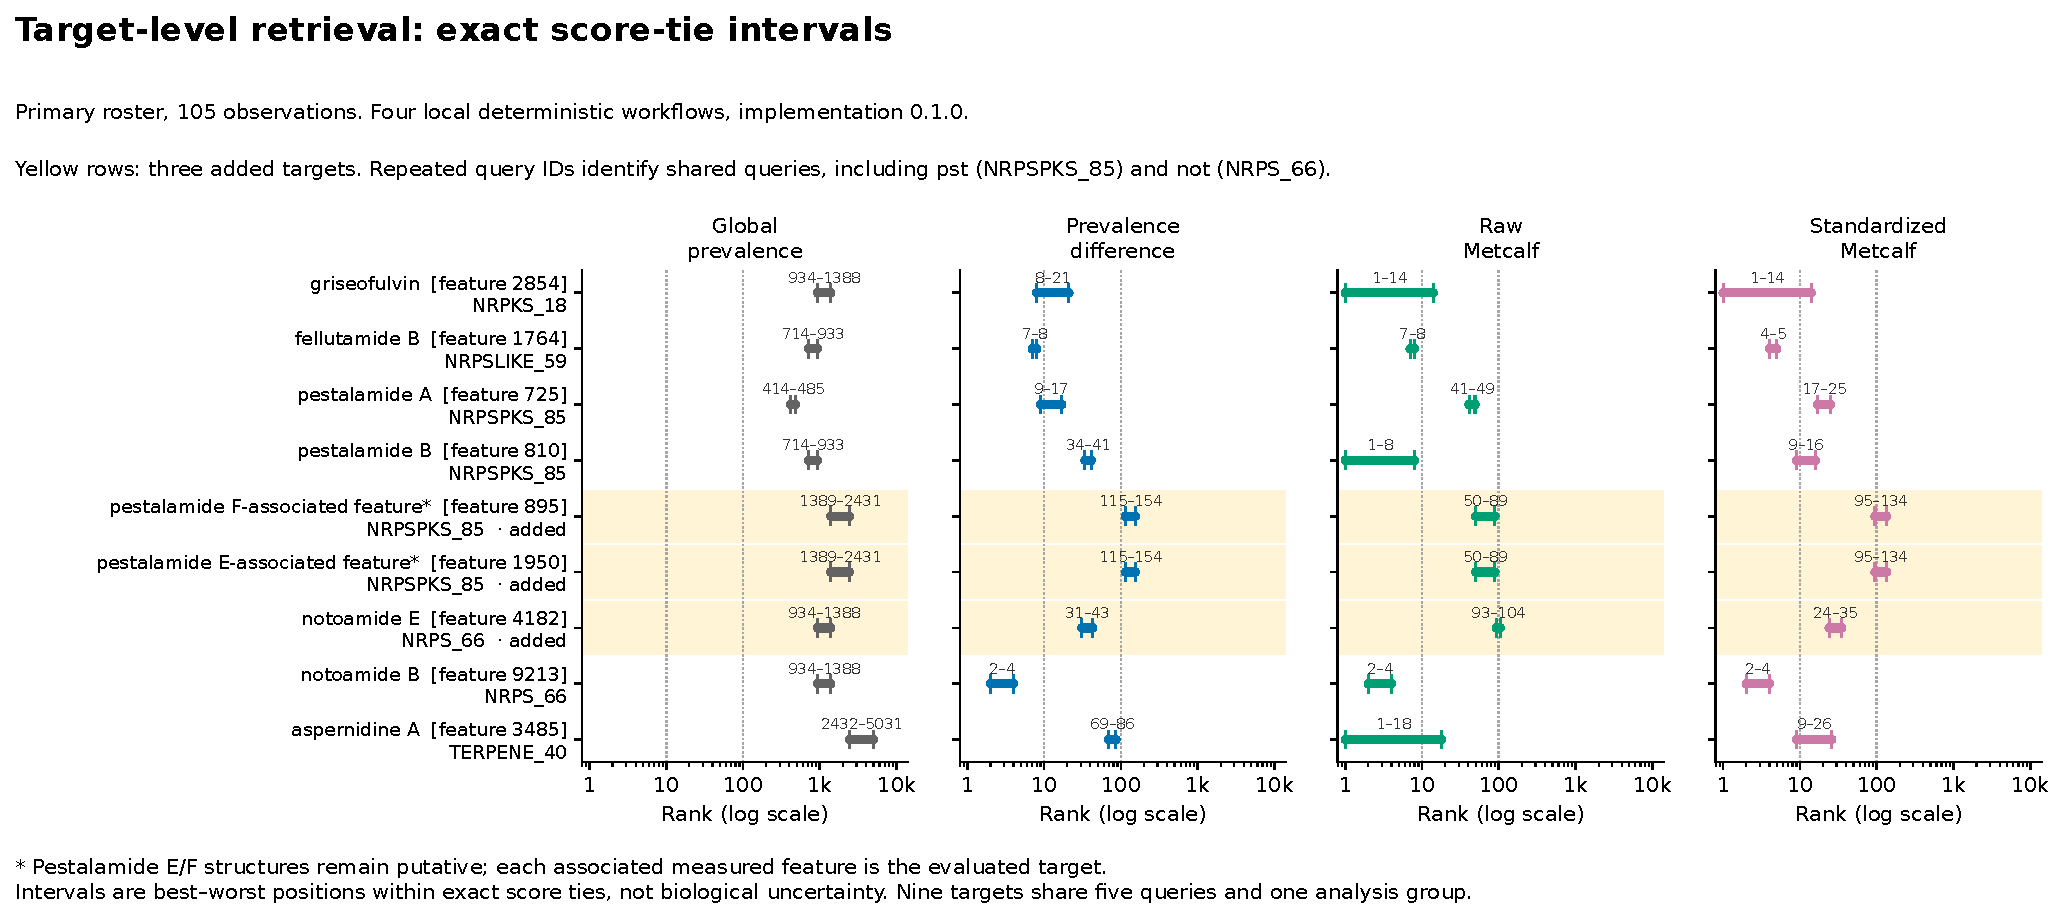
\includegraphics[width=\linewidth,height=0.62\textheight,keepaspectratio]{figures/Figure-S3.pdf}
\caption{Traceable target retrieval under the primary roster. Each interval gives the first and last possible rank of a supported singleton measured target within its exact score-tie block among 9,339 candidates. Facets show global prevalence, prevalence difference, raw Metcalf and standardized Metcalf, all local implementation version 0.1.0, for the primary 105-observation roster. Rank is logarithmic; dotted lines mark cutoffs 10 and 100. All 36 target-method intervals were independently recomputed from cached scores by counting candidates with greater and equal scores, then matched to evaluator product-rank records. Their cutoff probabilities were also checked. Yellow rows distinguish added notoamide E and the pestalamide E/F-associated features from the six original targets. Pestalamide E/F structure names remain putative; the declared measured-feature targets are evaluated without claiming exact structure elucidation. Repeated query IDs identify the four pst targets and two notoamide targets, so the nine rows represent five queries in one analysis group. For example, raw Metcalf places the E/F-associated features at ranks 50--89, while prevalence difference places them at 115--154; raw Metcalf places added notoamide E at 93--104, crossing the rank-100 cutoff. These illustrate recovery and nonrecovery at a declared cutoff, not validation of unsupported candidates. All cached scores remain unchanged.}
\label{fig:S3}
\end{figure}

\FloatBarrier

\end{document}
